\documentclass[11pt]{article}
\usepackage[round]{natbib}
\usepackage{graphicx}
\usepackage{listings}
\usepackage{caption}
\usepackage{subcaption}
\usepackage{pgf}
\usepackage[most]{tcolorbox}
\usepackage[margin=1in]{geometry}
\usepackage{xcolor}
\usepackage{inconsolata}
\usepackage{cleveref}
\usepackage[inline]{enumitem}
\usepackage{dcolumn}
\usepackage{booktabs}

\usepackage[scaled]{helvet}
\renewcommand\familydefault{\sfdefault}
\usepackage[T1]{fontenc}

\begin{document}

\definecolor{cyan}{RGB}{1, 132, 188}
\definecolor{blue}{RGB}{60, 120, 242}
\definecolor{purple}{RGB}{166, 38, 164}
\definecolor{green}{RGB}{80, 161, 79}
\definecolor{red1}{RGB}{228, 86, 73}
\definecolor{red2}{RGB}{202, 18, 67}
\definecolor{orange1}{RGB}{152, 104, 1}
\definecolor{orange2}{RGB}{193, 132, 1}

\definecolor{background}{RGB}{250, 250, 250}

\definecolor{mono1}{RGB}{56, 58, 66}
\definecolor{mono2}{RGB}{105, 108, 119}
\definecolor{mono3}{RGB}{160, 161, 167}

% \definecolor{lightgray}{rgb}{.9,.9,.9}
% \definecolor{darkgray}{rgb}{.4,.4,.4}
% \definecolor{purple}{rgb}{0.65, 0.12, 0.82}
% \definecolor{atomred}{RGB}{224, 108, 117}
% \definecolor{atomwhite}{RGB}{250, 250, 250}
% \definecolor{atomorange}{RGB}{}

\lstdefinelanguage{JavaScript}{
  keywords={typeof, new, true, false, catch, function, return, null, catch, switch, var, if, in, while, do, else, case, break, class, export, boolean, throw, implements, import, this},
  sensitive=false,
  comment=[l]{//},
  morecomment=[s]{/*}{*/},
  morestring=[b]',
  morestring=[b]"
}

\lstset{
  backgroundcolor=\color{background},
  basicstyle=\ttfamily\footnotesize,
  breakatwhitespace=false,
  breaklines=true,
  captionpos=b,
  commentstyle=\color{mono3}\ttfamily,
  extendedchars=true,
  frame=single,
  keepspaces=true,
  keywordstyle=\color{purple}\bfseries,
  language=Bash,
  numbers=left,
  numbersep=5pt,
  numberstyle=\tiny\color{mono1},
  rulecolor=\color{black},
  showspaces=false,
  showstringspaces=false,
  showtabs=false,
  stepnumber=1,
  stringstyle=\color{green}\ttfamily,
  tabsize=2,
  title=\lstname
}

\lstset{
  backgroundcolor=\color{background},
  basicstyle=\ttfamily\footnotesize,
  breakatwhitespace=false,
  breaklines=true,
  captionpos=b,
  commentstyle=\color{mono3}\ttfamily,
  extendedchars=true,
  frame=single,
  keepspaces=true,
  keywordstyle=\color{purple}\bfseries,
  language=JavaScript,
  numbers=left,
  numbersep=5pt,
  numberstyle=\tiny\color{mono1},
  rulecolor=\color{black},
  showspaces=false,
  showstringspaces=false,
  showtabs=false,
  stepnumber=1,
  stringstyle=\color{green}\ttfamily,
  tabsize=2,
  title=\lstname
}


\title{On the Performance of String Search Algorithms for Deep Packet Inspection - Followup}
\author{Kieran Hunt}
\date{\today}
\maketitle

%TODO: Abstract

\section{Introduction}

In an earlier paper, \citet{hunt2016} compares various string search algorithms for use in Deep Packet Inspection (DPI). This paper serves as an extension to that work; it follows up on a few select algorithms. 

From that earlier paper the following algorithms were selected: Horspool \citep{horspool1980}, QuickSearch \citep{sunday1990}, NotSoNaive \citep{hancart1993}, and RabinKarp \citep{karp1987}.

For each of the selected algorithms the following questions were posed:
\begin{itemize}
  \item How does the length of a packet's payload affect the speed at which that packet is processed?
  \item How does the number of matches found within a packet affect the speed at which that packet is processed?
  \item How does the number of threads used when performing the matching affect the speed at which a packet is processed?
\end{itemize}
 
 From these questions the following paper has been created.

\subsection{Algorithms}

In \citep{hunt2016}, the authors compare a number string search algorithms against each other. From their results we have chosen the two best and two worst performing algorithms. The two best performing algorithms - based on their mean processing times - were the Horspool \citep{horspool1980} and QuickSearch \citep{sunday1990}; the two worst performing - based on the same criterion - were NotSoNaive \citep{hancart1993} and RabinKarp \citep{karp1987}. Table \ref{table-algorithms} presents these algorithms along with the year they were published, their authors, and the time complexity associated with each one. 

\begin{table}[!hbt]
\centering
\begin{tabular}{@{}llll@{}}
  \toprule
  Algorithm & Year & Author(s) & Time Complexity \\ \midrule
  Horspool & \citeyear{horspool1980} & \citeauthor{horspool1980} & O(n + m) \\
  RabinKarp & \citeyear{karp1987} & \citeauthor{karp1987} & O(mn) \\
  QuickSearch & \citeyear{sunday1990} & \citeauthor{sunday1990} & O(mn) \\
  NotSoNaive & \citeyear{hancart1993} & \citeauthor{hancart1993} & O(nm) \\ \bottomrule
 \end{tabular}
\caption{String search algorithms. Under time complexity, \textit{n} represents the length of the input and \textit{m} represents the length of a rule.}
\label{table-algorithms}
\end{table}

\subsection{Datasets}

Table \ref{table-datasets} presents the datasets used throughout the rest of the paper. In Table \ref{table-datasets}, '$\mu$ Length' refers the mean length of the inputs, in bytes, within that dataset and '\# Inputs' refers to the number of inputs in that dataset. An input is defined as a Both \textit{Dataset A} and \textit{Dataset B} have been reused from the earlier datasets used in \citet{hunt2016}.

\begin{table}[!htb]
\centering
\begin{tabular}{@{}lp{0.5\textwidth}ll@{}}
\toprule
Name & Description & $\mu$ Length & \# Inputs \\ \midrule
\textit{Dataset A} & Real-world DNS traffic & 109.61 & 10000 \\
\textit{Dataset B} & Full text of \textit{Alice in Wonderland} by Lewis Carroll & 163780 & 1 \\
\textit{Dataset C} & Randomly generated DNS traffic with a payload size between 0 and 1500 bytes & 770.89 & 10000 \\
\textit{Dataset D} & Dataset C edited so that the payload just contains matches to the required rules & 770.89 & 10000 \\
\textit{Dataset E} & Dataset C edited so that each packet is filled with a random number of matches & 769.92 & 10000 \\
\textit{Dataset F} & Packets of fixed length - filled with a random number of matches & 1500 & 10000 \\ \bottomrule
\end{tabular}
\caption{All datasets used in the tests}
\label{table-datasets}
\end{table}

\textit{Dataset C} was created using Wireshark's\footnote{https://www.wireshark.org/} \texttt{randpkt} tool \citep{randpkt2016}. Listing \ref{listing-randpkt-dns} shows how that Dataset was created.

\begin{lstlisting}[language = Bash, caption=Creating 10000 random DNS packets, label=listing-randpkt-dns]
$ randpkt -b 1500 -c 10000 -t dns random_dns.pcap
\end{lstlisting}

The packets in \textit{Dataset C} had an average length of 770 bytes as can be seen in Table \ref{table-datasetcinputlengthsummary}. As \textit{Dataset C} was completely comprised of random bytes, the number of matches within it was near zero. This dataset was useful when comparing processing speed with input length as the number of matches within each packet would not affect the processing speed.

\begin{table}[!htb]
\centering
\begin{tabular}{@{}llllll@{}}
\toprule
Min & First Quartile & Median & Mean & Third Quartile & Max \\ \midrule
44 & 407 & 763.5 & 770.9 & 1136 & 1500 \\ \bottomrule
\end{tabular}
\caption{A summary of the input lengths in \textit{Dataset C}}
\label{table-datasetcinputlengthsummary}
\end{table}

\textit{Dataset D} was a modification of \textit{Dataset C}. To make \textit{Dataset D}, \textit{Dataset C} was edit such that each packet's payload was combination of each the rules. For each packet, a list of the rules would have its order randomised, the list would then be turned into a string and then string multiplied until its length was greater than that of the packet's payload, the string would then be truncated to the length of the packet's payload and the packet would be edited so that its payload is that string. The result of these changes to \textit{Dataset C} means that each packet - although of random length - is completely filled with matches to the rules used in the tests.

\textit{Dataset E} was also a modification of \textit{Dataset C}. Unlike \textit{Dataset D}, \textit{Dataset E} contains a random amount of matches to the rules and the rest of the space is filled with random bytes. The construction of \textit{Dataset E} is similar to that of \textit{Dataset D}. Prior to changing the packet's payload to the string of matches a random number is calculated. That random number is between zero and the length of the packet's payload. The string of matches is then truncated to the length of that random number, the packet's payload is updated to contain that string and then the subsequent bytes from the random number to the original length of the packet's payload is filled randomly.

\textit{Dataset F} was constructed as a way to isolate the number of matches from the length of the packet's payload. For this dataset all packets were created with a length of 1500 bytes. Like with \textit{Dataset E}, each packet would be filled with a random number of matches and the rest of the space in the payload would be filled with random bytes. The result is a dataset with packets of 1500 bytes in length and a random number of matches within each.

\section{Processing Speed vs Input Length} \label{sec-processingspeecvsinputlength}

In \citet{hunt2016}, the Dataset used by the authors (\textit{Dataset A}) contains matches to the rules being searched for. For some algorithms the number of matches may affect the processing speed of each packet. Furthermore, \textit{Dataset A}'s shortfall is that - because it contains real-world DNS data - the average length of a packet is very short (See Table \ref{table-datasets}). \textit{Dataset C} was created for for the purpose of this test as it contains packets of much longer length with zero matches to the rules used in the tests.

For this test the processing speed of each packet is now independent of the number of matches as the number of matches has been reduced to zero.

Each of the four algorithms were tested for the same rules as in \citet{hunt2016} and with \textit{Dataset C} as input. Figure \ref{figure-individualalgorithmsvslength} shows a comparison between each of the algorithms.


\begin{figure}[!htb]
  \centering
  \begin{subfigure}[b]{0.48\textwidth}
      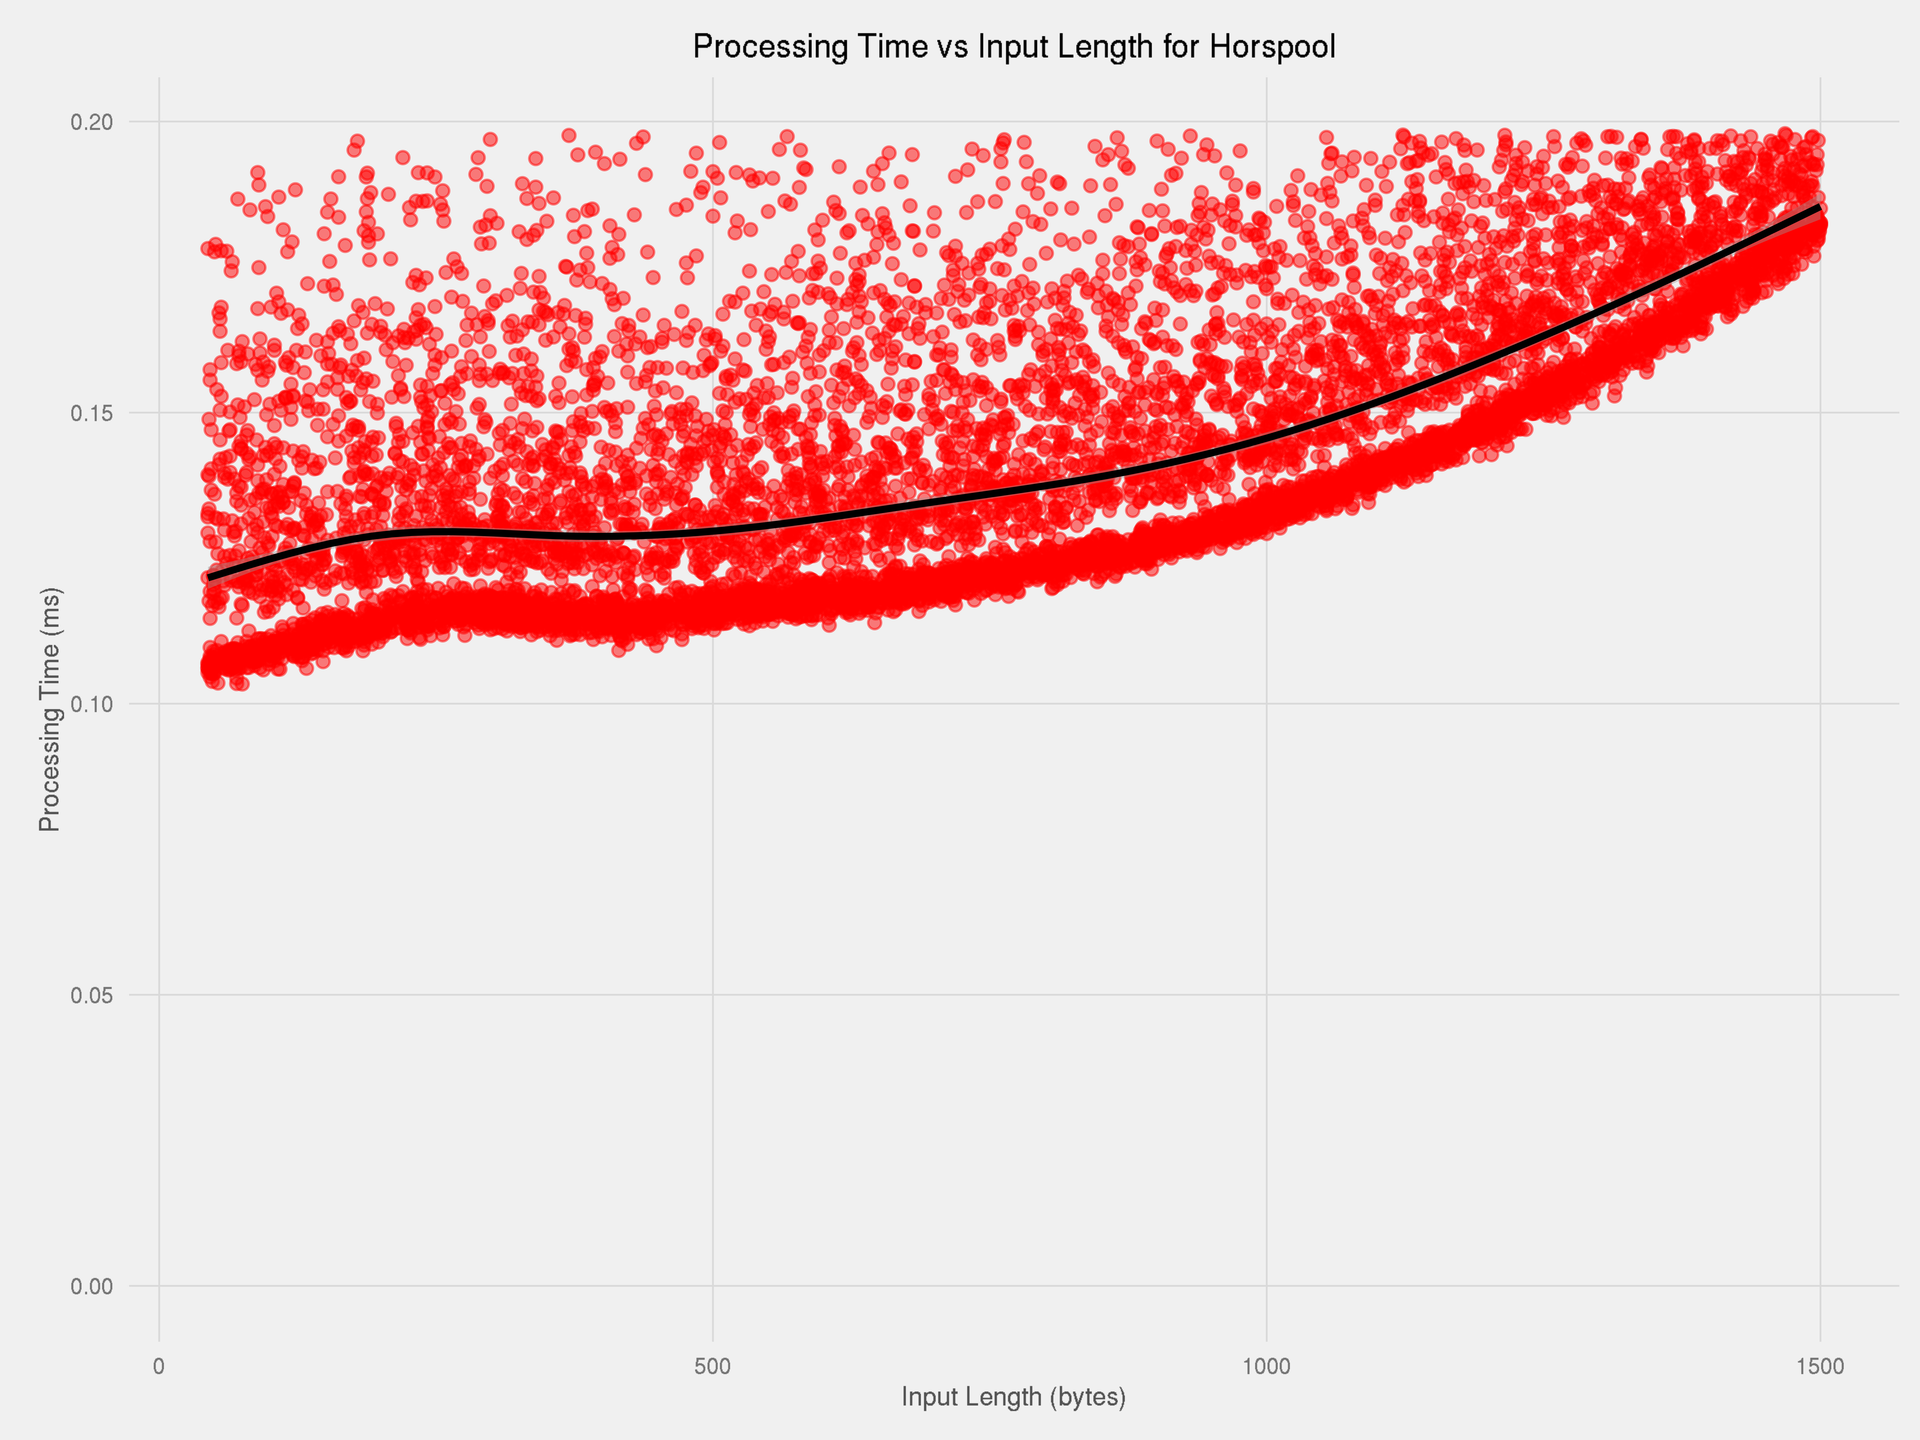
\includegraphics[width=\textwidth]{images/processing_speed_vs_input_length_no_matches_Horspool}
      \caption{Horspool}
      \label{figure-processingtimevslengthhorspool}
  \end{subfigure}
  \begin{subfigure}[b]{0.48\textwidth}
      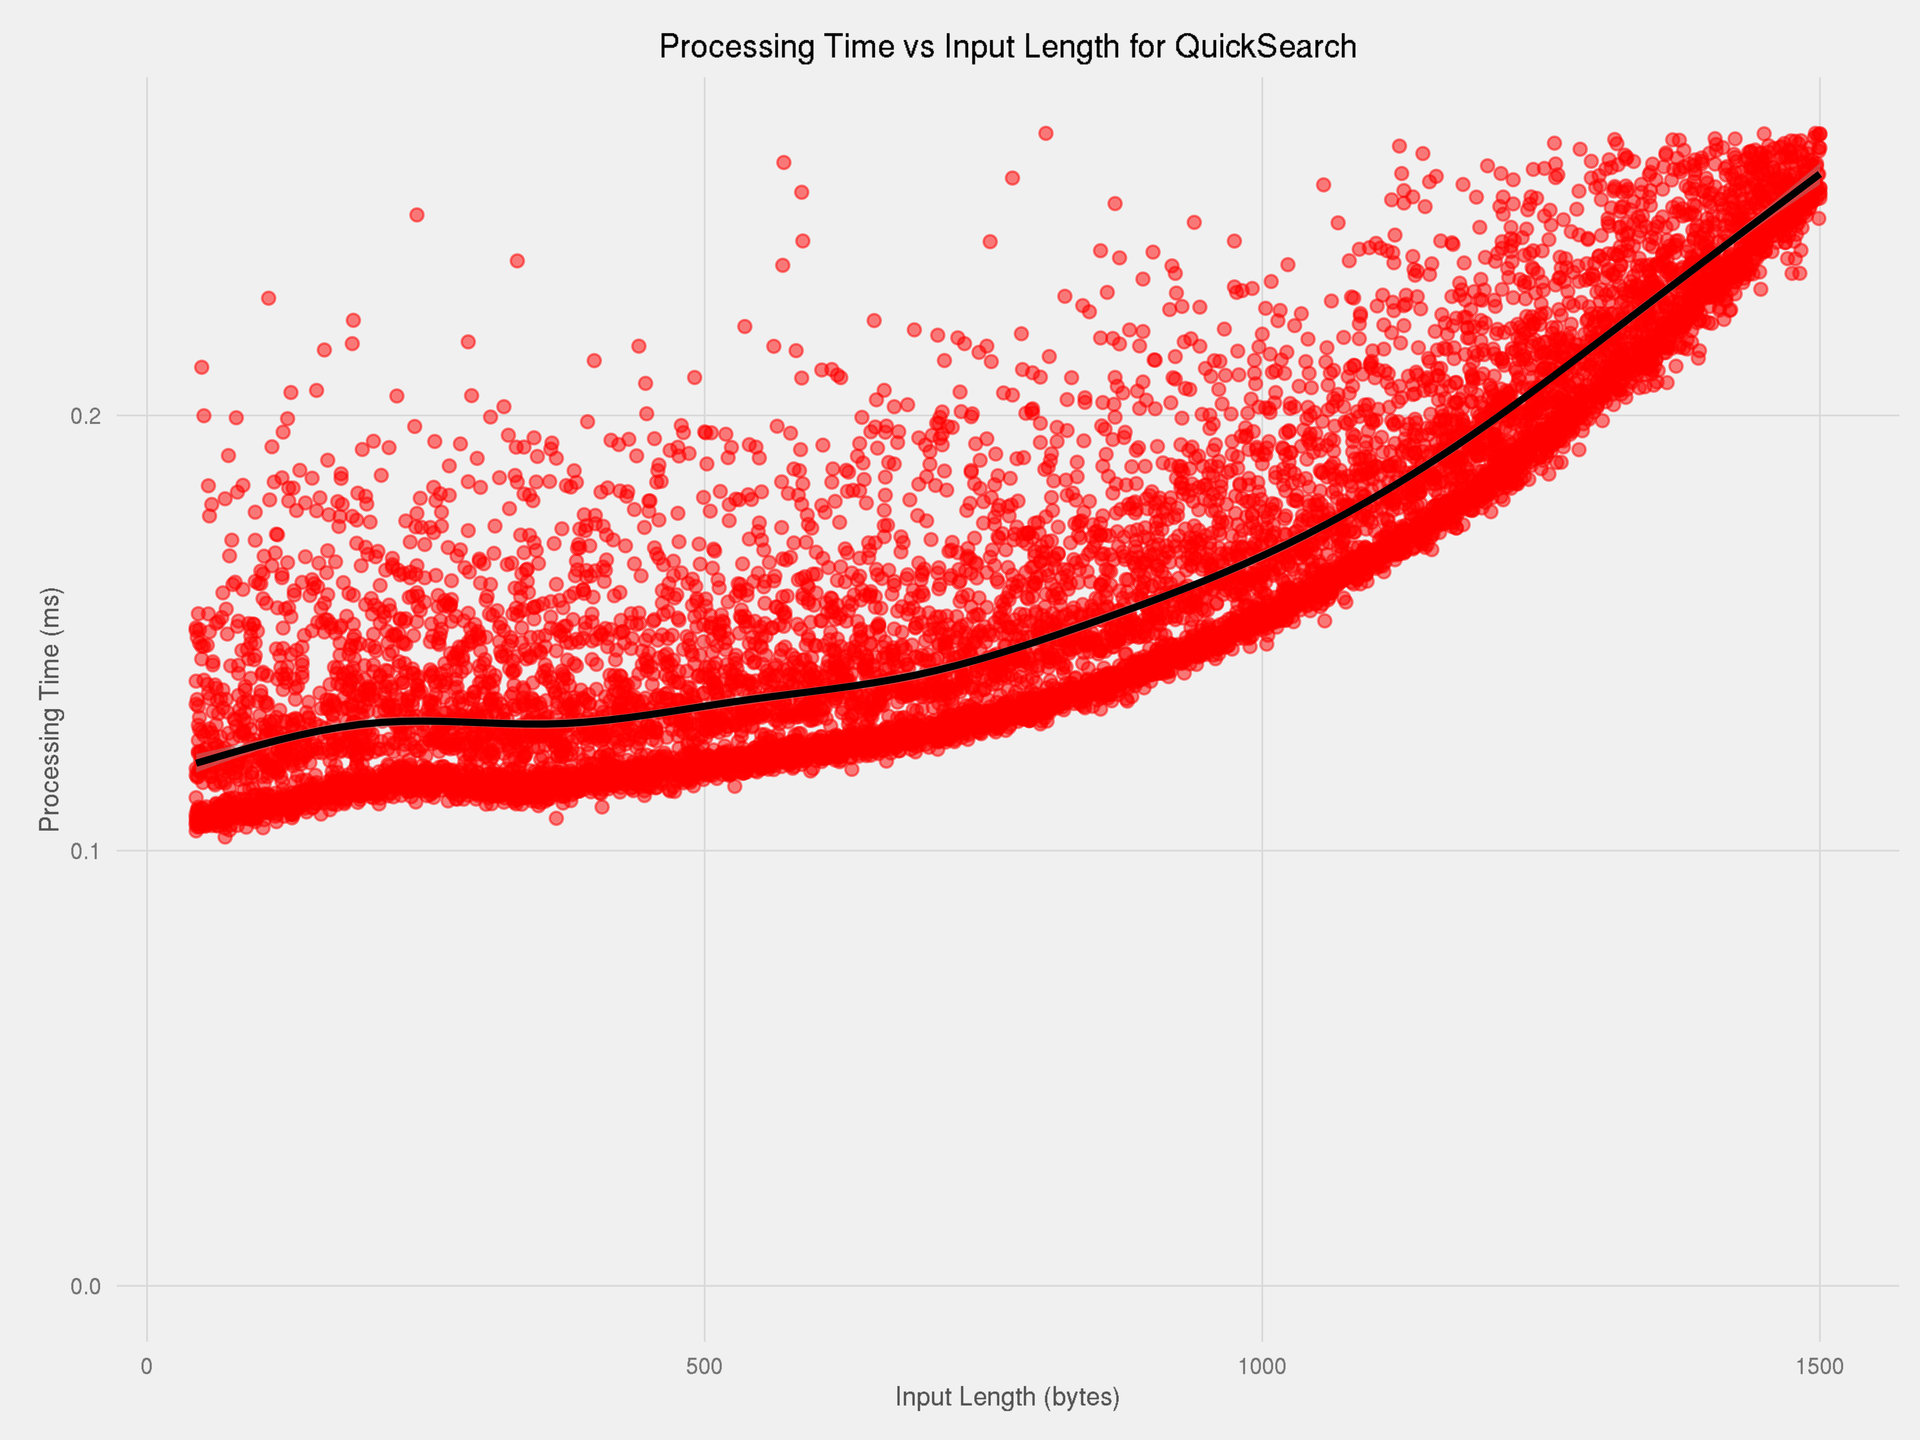
\includegraphics[width=\textwidth]{images/processing_speed_vs_input_length_no_matches_QuickSearch}
      \caption{QuickSearch}
      \label{figure-processingtimevslengthquicksearch}
  \end{subfigure}
  ~
  \begin{subfigure}[b]{0.48\textwidth}
      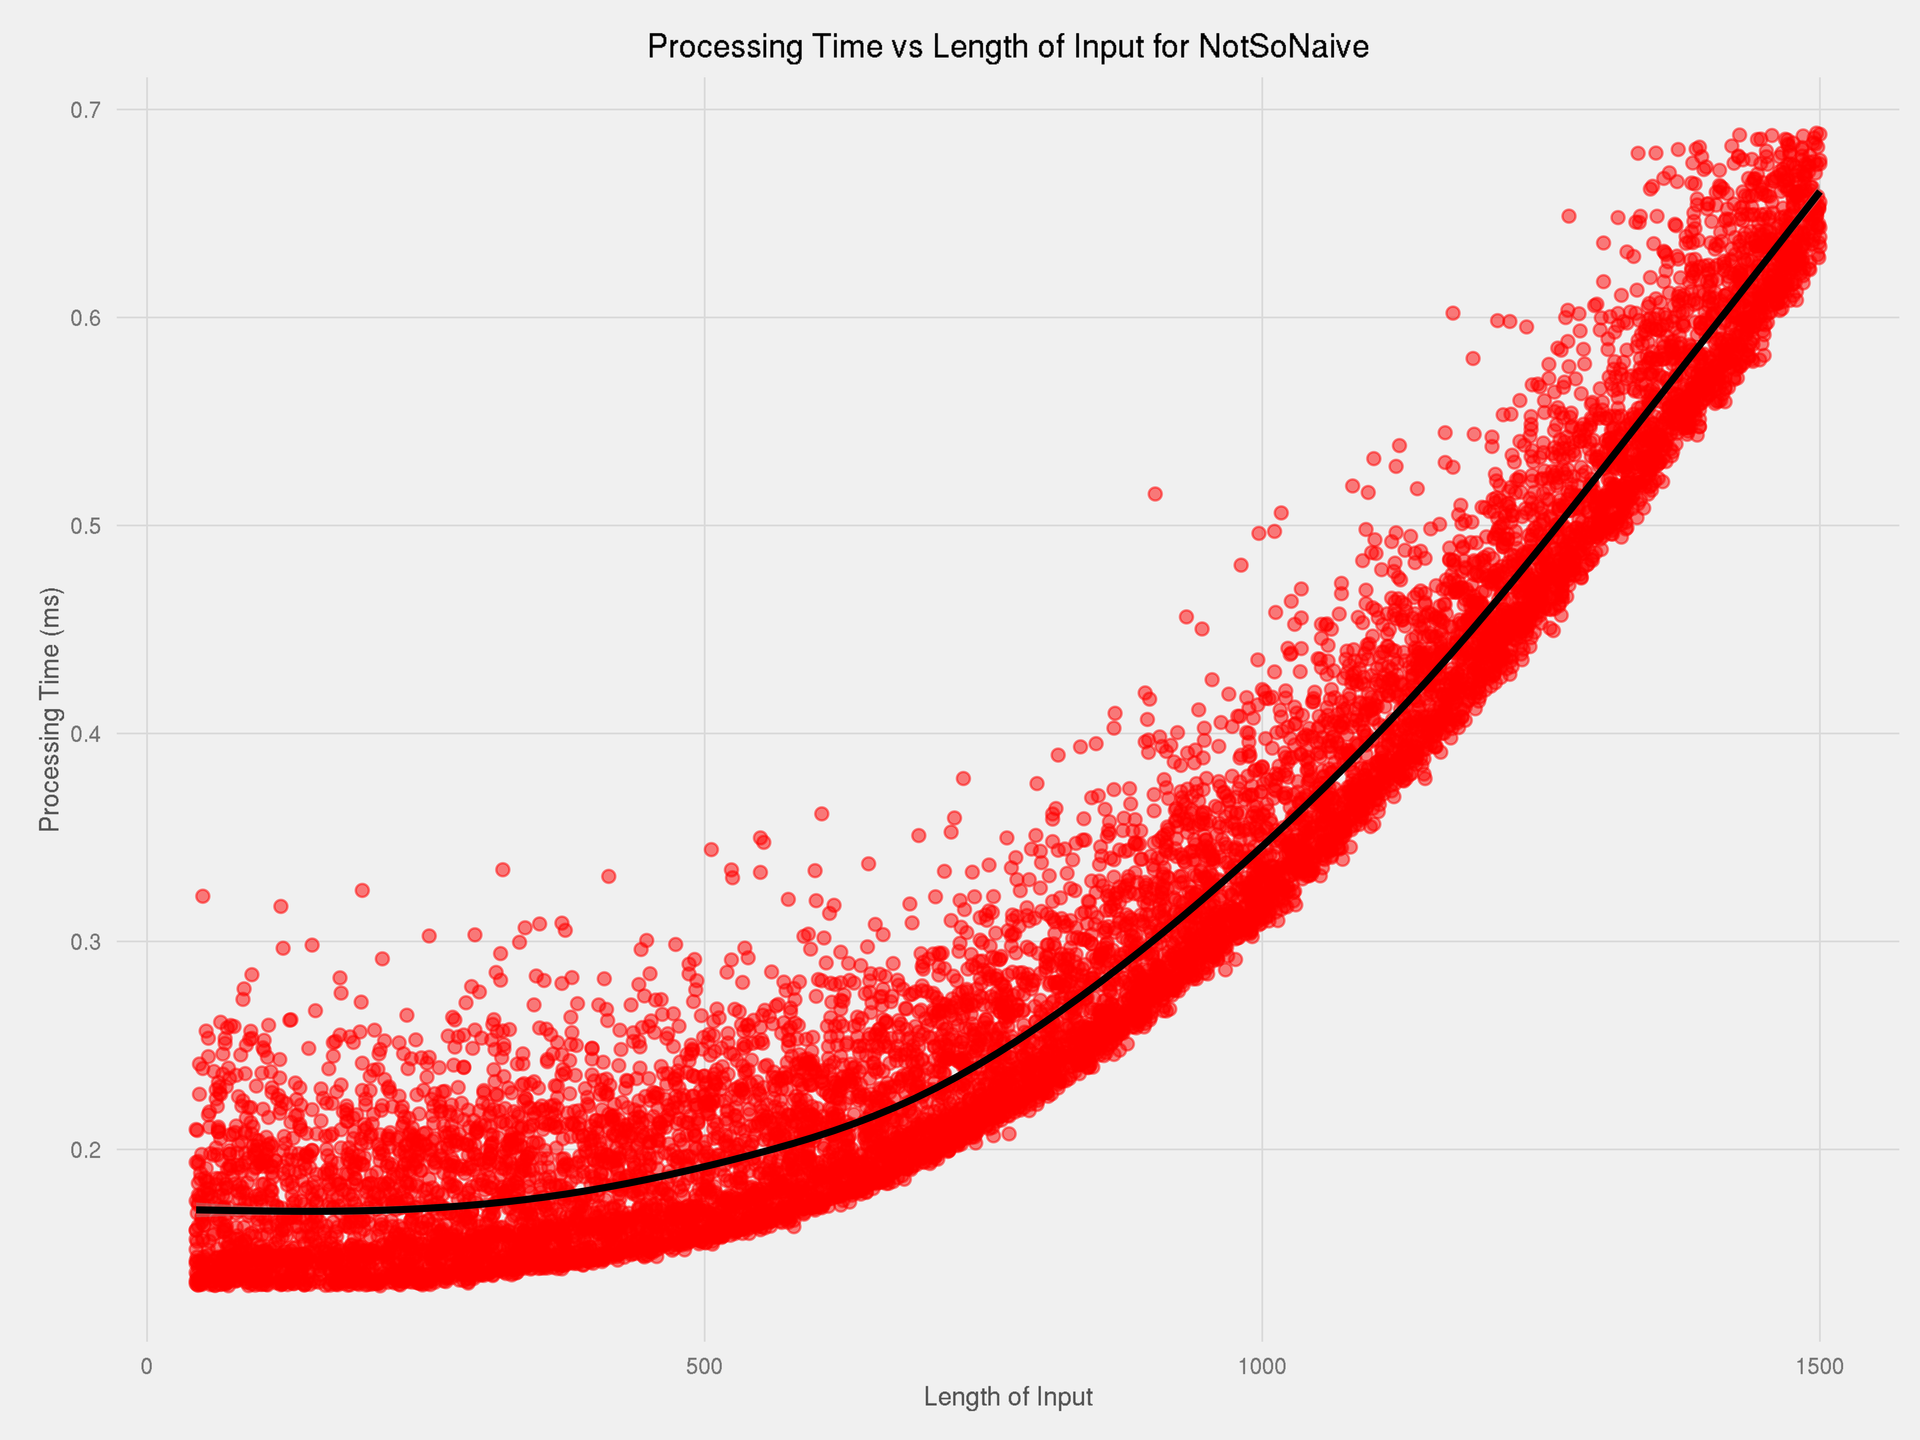
\includegraphics[width=\textwidth]{images/processing_speed_vs_input_length_no_matches_NotSoNaive}
      \caption{NotSoNaive}
      \label{figure-processingtimevslengthnotsonaive}
  \end{subfigure}
  \begin{subfigure}[b]{0.48\textwidth}
      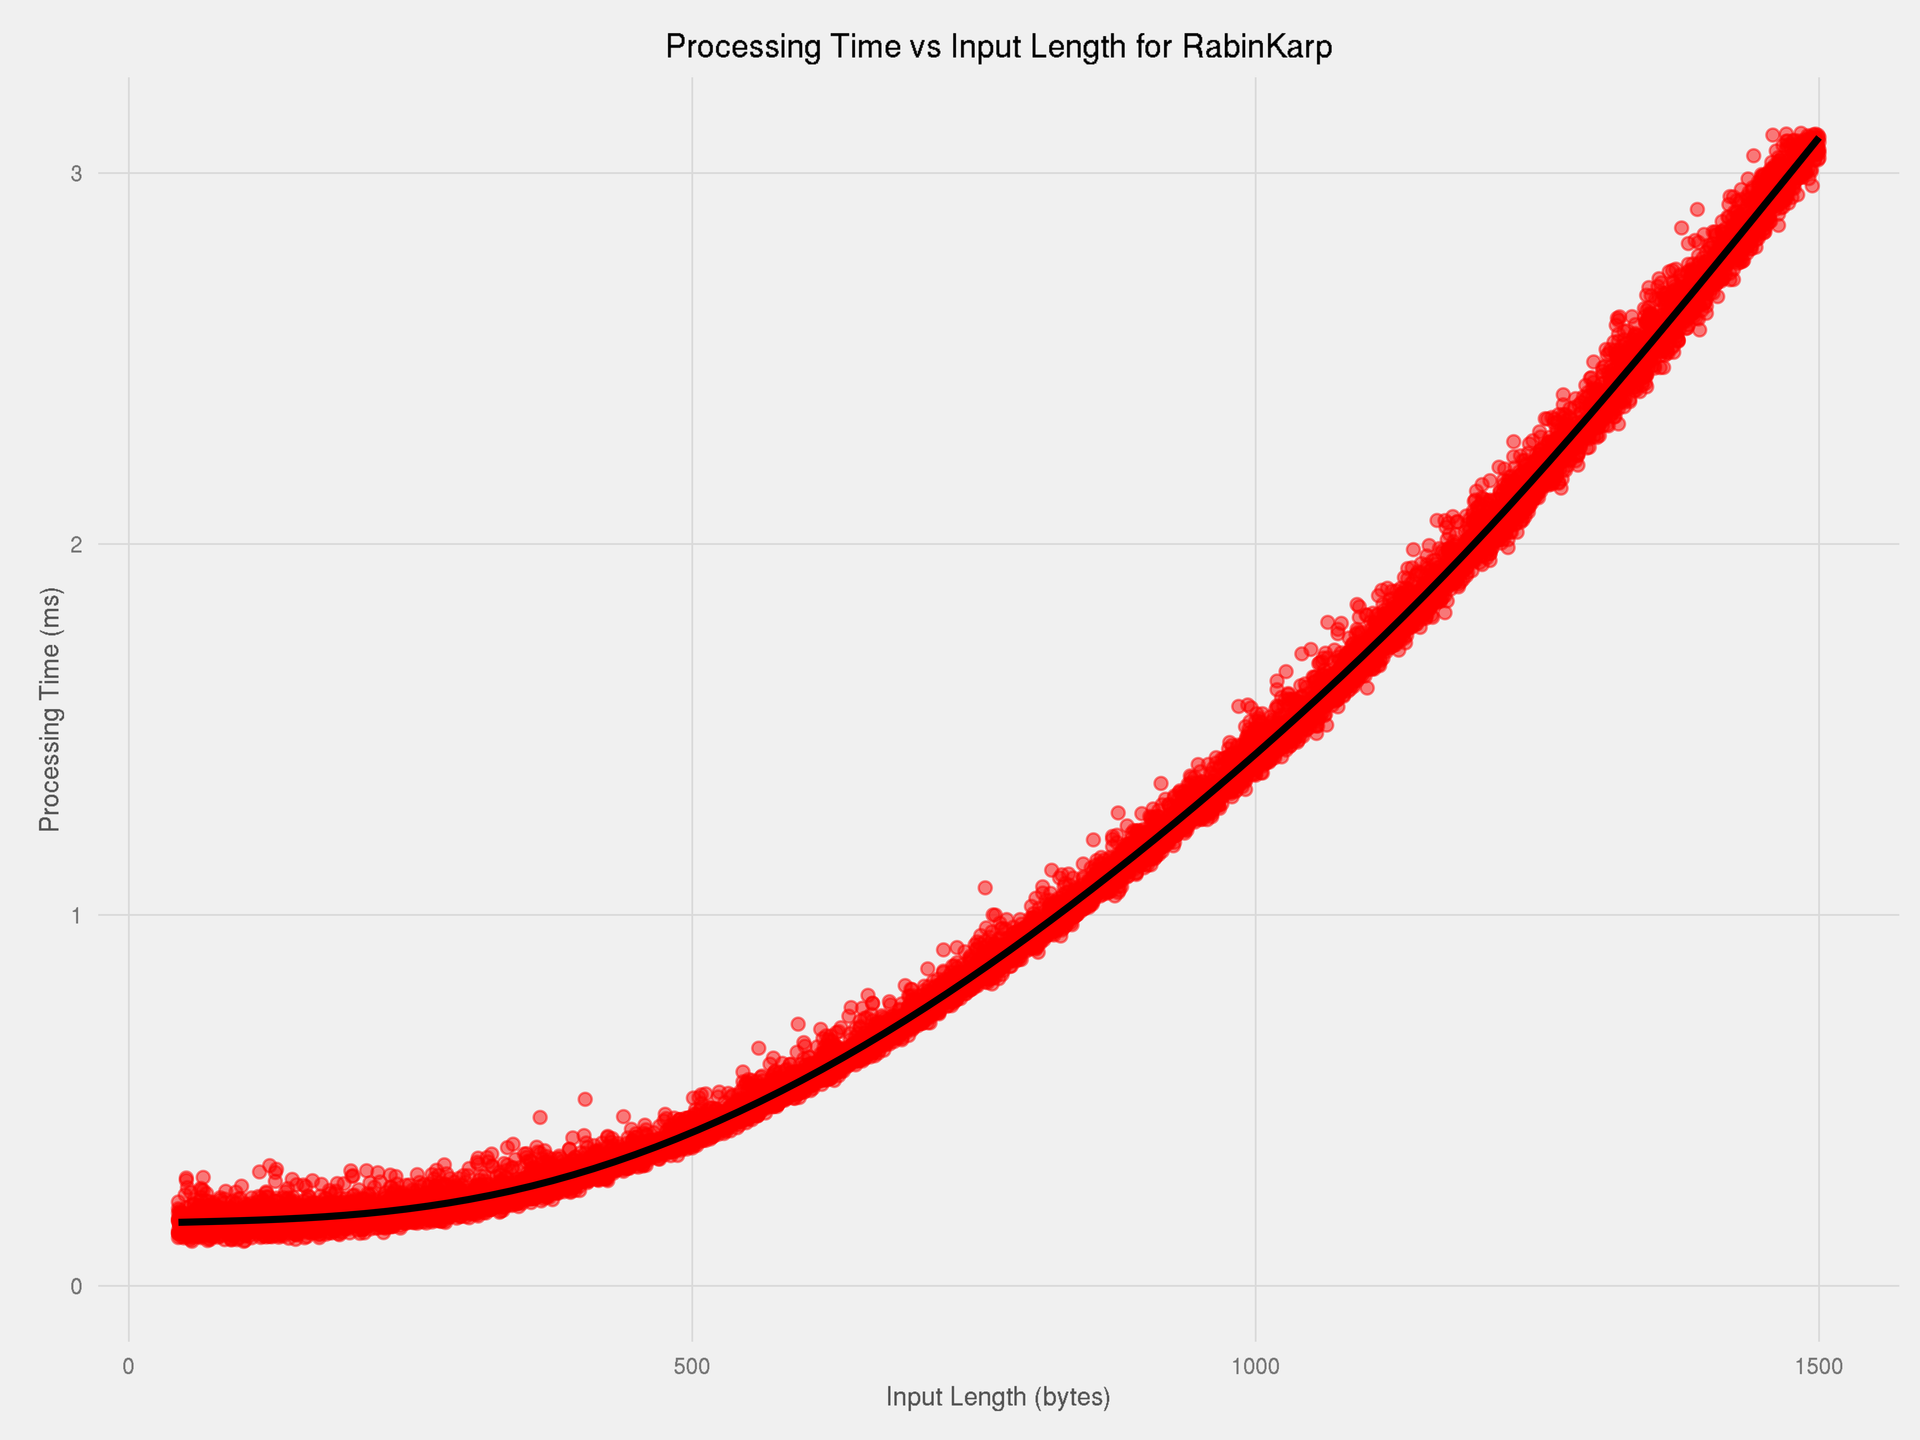
\includegraphics[width=\textwidth]{images/processing_speed_vs_input_length_no_matches_RabinKarp}
      \caption{RabinKarp}
      \label{figure-processingtimevslengthrabinkarp}
  \end{subfigure}
  \caption{Mean processing times versus input length for the Horspool, QuickSearch, NotSoNaive, and RabinKarp algorithms for \textit{Dataset C}.}
  \label{figure-individualalgorithmsvslength}
\end{figure}

From Figure \ref{figure-individualalgorithmsvslength}, it is clear that the processing times for Horspool and QuickSearch (Subfigures \ref{figure-processingtimevslengthhorspool} and \ref{figure-processingtimevslengthquicksearch} respectively) do not rise as quickly as those of NotSoNaive and RabinKarp (Subfigures \ref{figure-processingtimevslengthnotsonaive} and \ref{figure-processingtimevslengthrabinkarp} respectively) for inputs of greater length. Both NotSoNaive and RabinKarp show an exponential rise in processing times. Another point to note is that the maximum processing time for NotSoNaive is almost 3 times that of Horspool and QuickSearch, and the maximum processing speed of Horspool is almost 5 times that of NotSoNaive.

Horspool and QuickSearch also show initial humps in processing speed around the 250 byte mark. This can be attributed to the overheard associated with each packet. For packets of more than 250 bytes, the processing speed relies more on the length of the packet then the initial - per-packet - overhead. This initial hump is not evident on either NotSoNaive nor RabinKarp; the reason for this is twofold. First, the speed of these algorithms is more affected by the input length, because of this an initial hump would be surpassed by the time it takes to process each packet. Second, the vertical scale of these two graphs is much larger than that Horspool or QuickSearch. Owing to that a small hump earlier on is less visible on a larger scale.


\section{Processing Speed vs Number of Matches}

For Section \ref{sec-processingspeecvsinputlength}, \textit{Dataset C} was created. It was designed in such a way that the number of matches in the input would not affect the processing speed. The processing speed was thus only affected by the length of the input and the algorithm used. In order to compare the processing speed against different numbers of matches, another dataset needed to be created. \textit{Dataset F} was created in such a way that the processing speed would only be affected by the number of matches and not the length of the packet. Each packet in this data set is 1500 bytes long.

Figure \ref{figure-individualalgorithmsvsnumberofmatches} presents the results for each algorithm of a comparison between the processing speed vs the number of matches in the packet.

\begin{figure}[!htb]
  \centering
  \begin{subfigure}[b]{0.48\textwidth}
      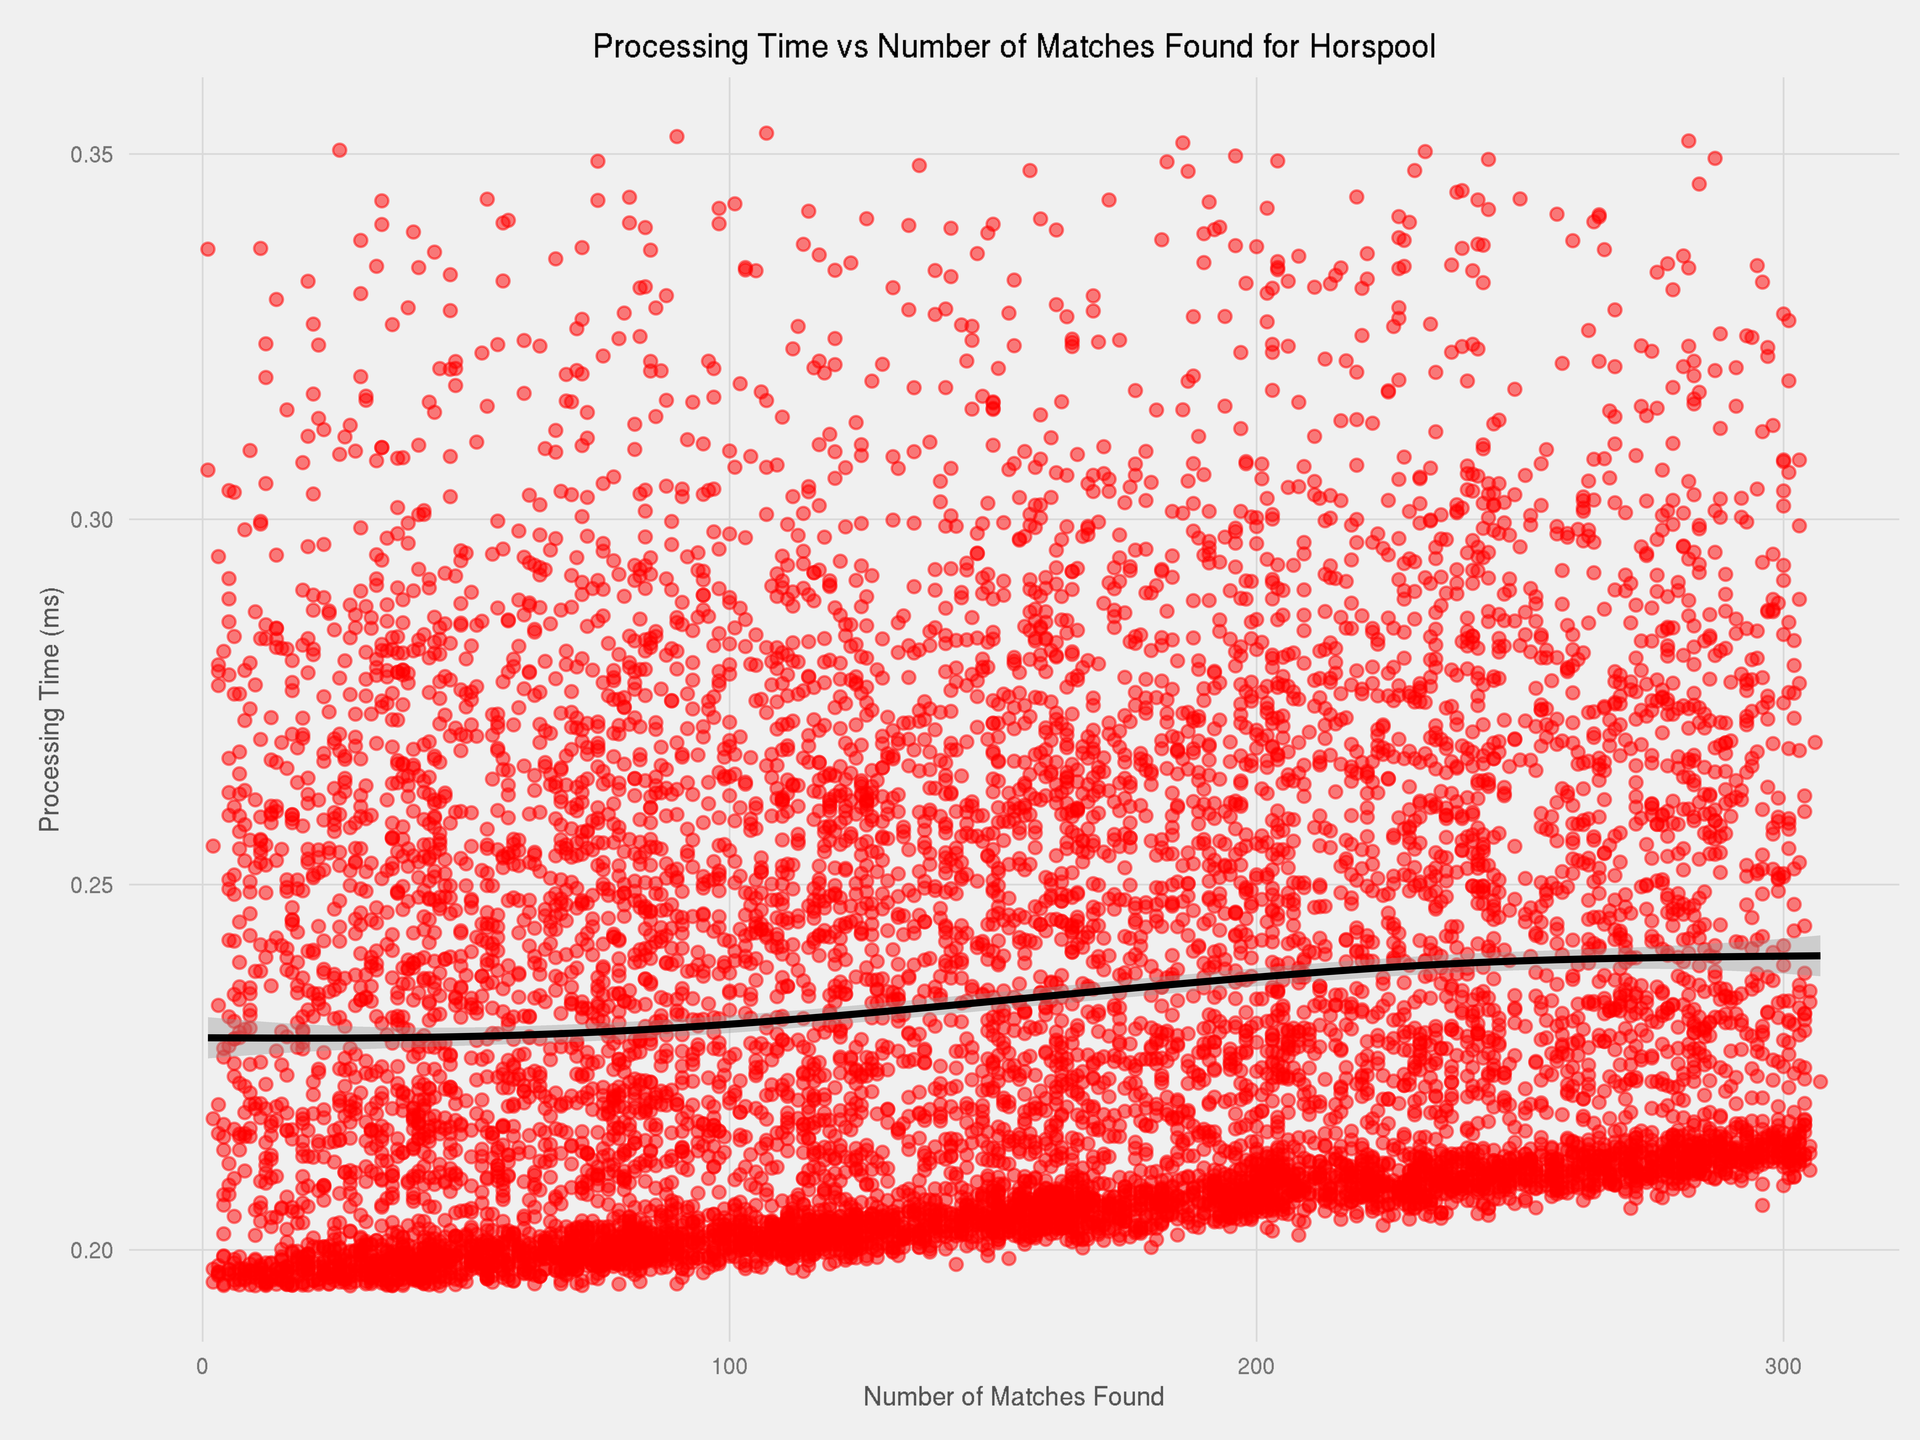
\includegraphics[width=\textwidth]{images/processing_speed_vs_num_matches_Horspool}
      \caption{Horspool}
  \end{subfigure}
  \begin{subfigure}[b]{0.48\textwidth}
      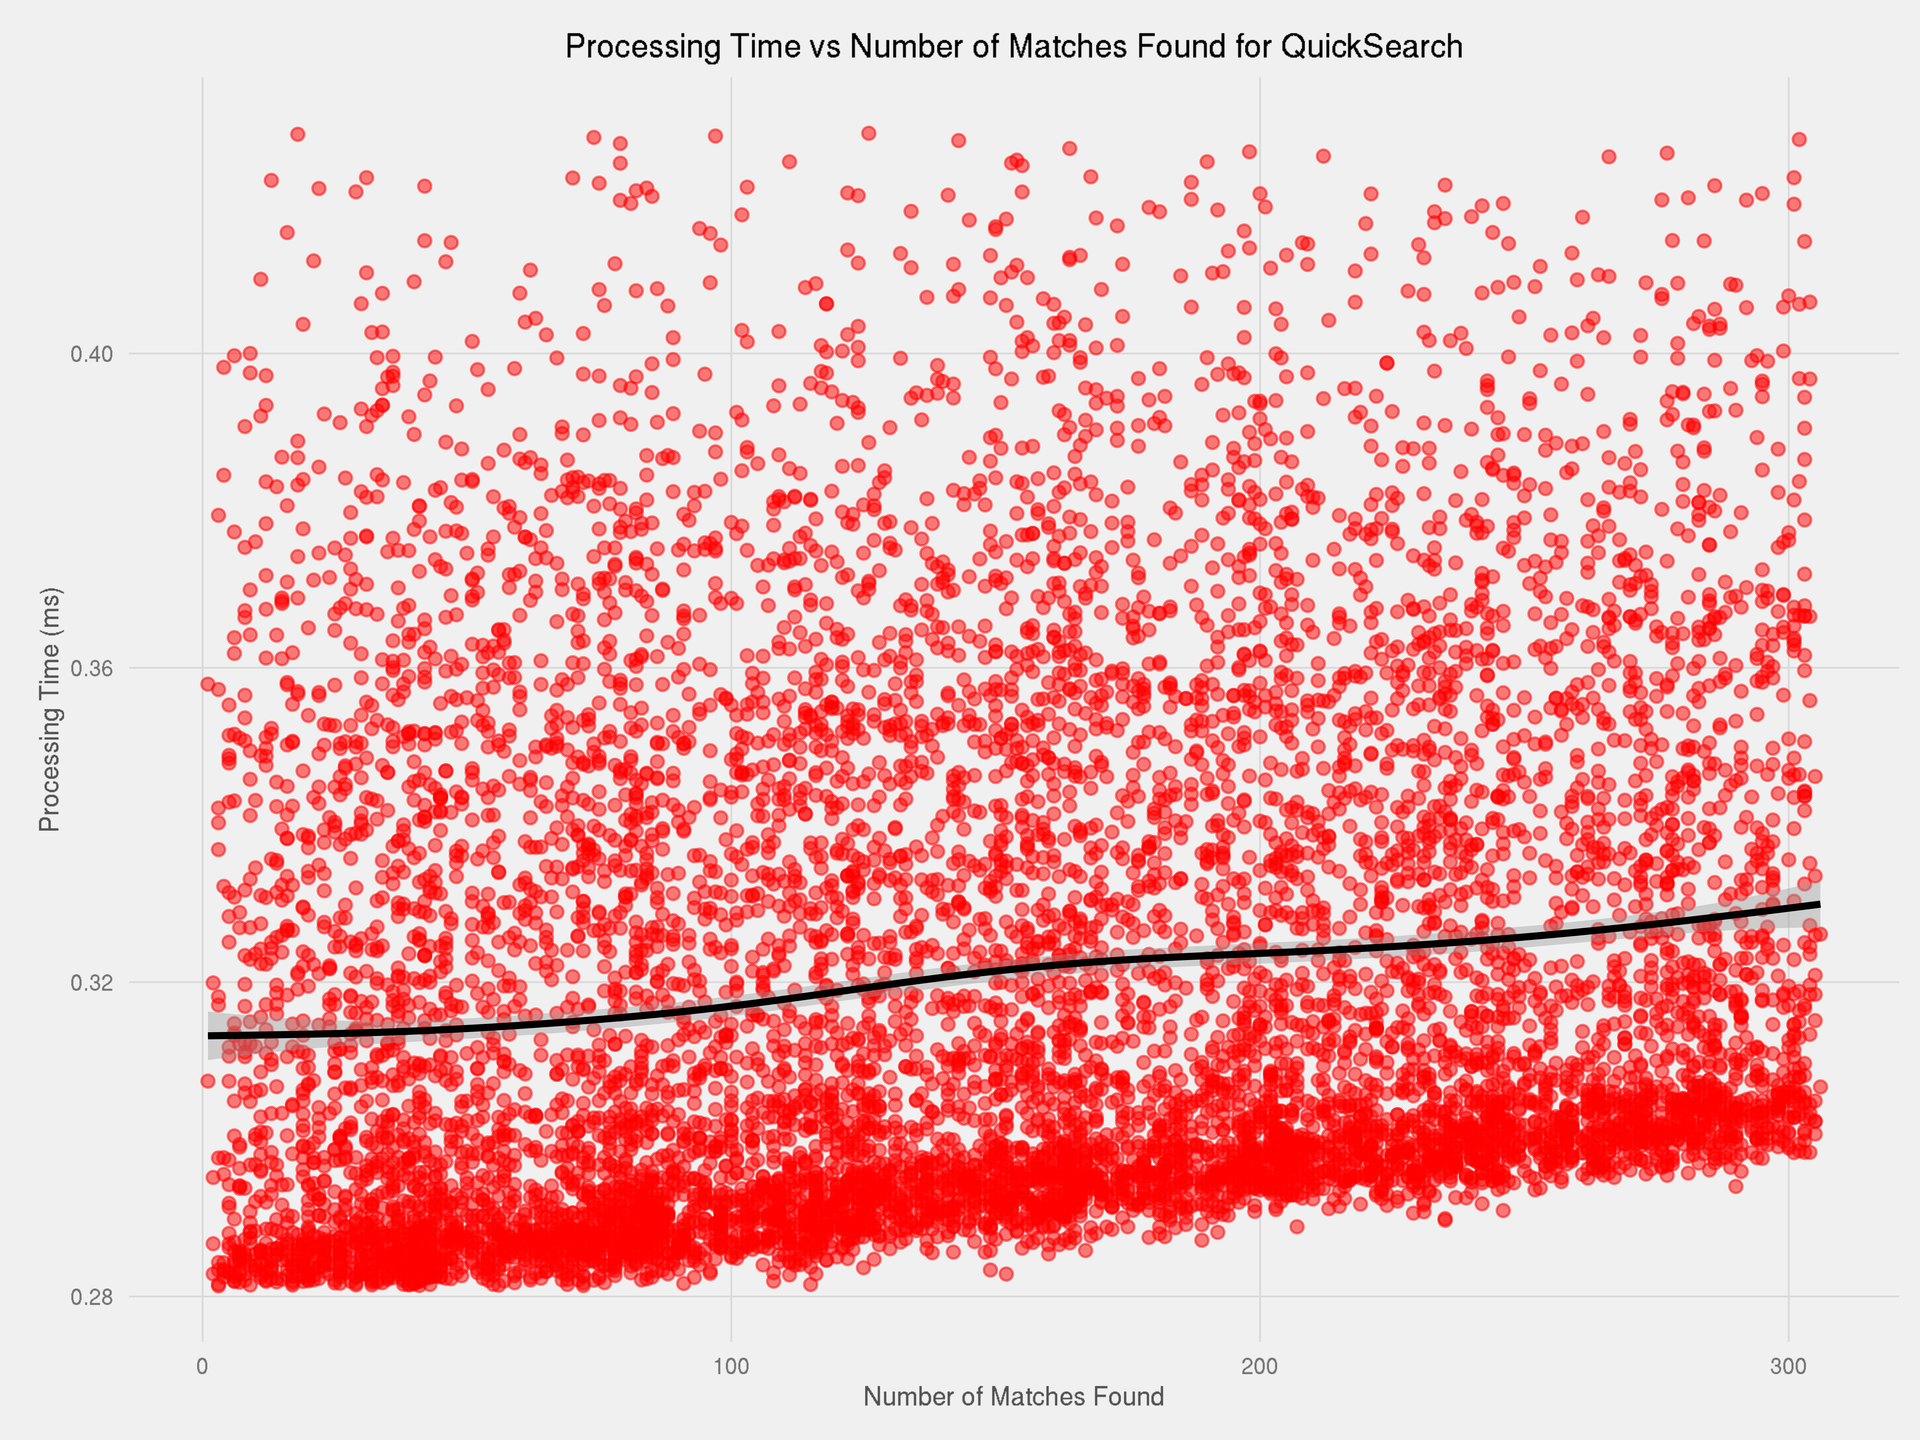
\includegraphics[width=\textwidth]{images/processing_speed_vs_num_matches_QuickSearch}
      \caption{QuickSearch}
  \end{subfigure}
  ~
  \begin{subfigure}[b]{0.48\textwidth}
      \includegraphics[width=\textwidth]{images/processing_speed_vs_num_matches_NotSoNaive}
      \caption{NotSoNaive}
  \end{subfigure}
  \begin{subfigure}[b]{0.48\textwidth}
      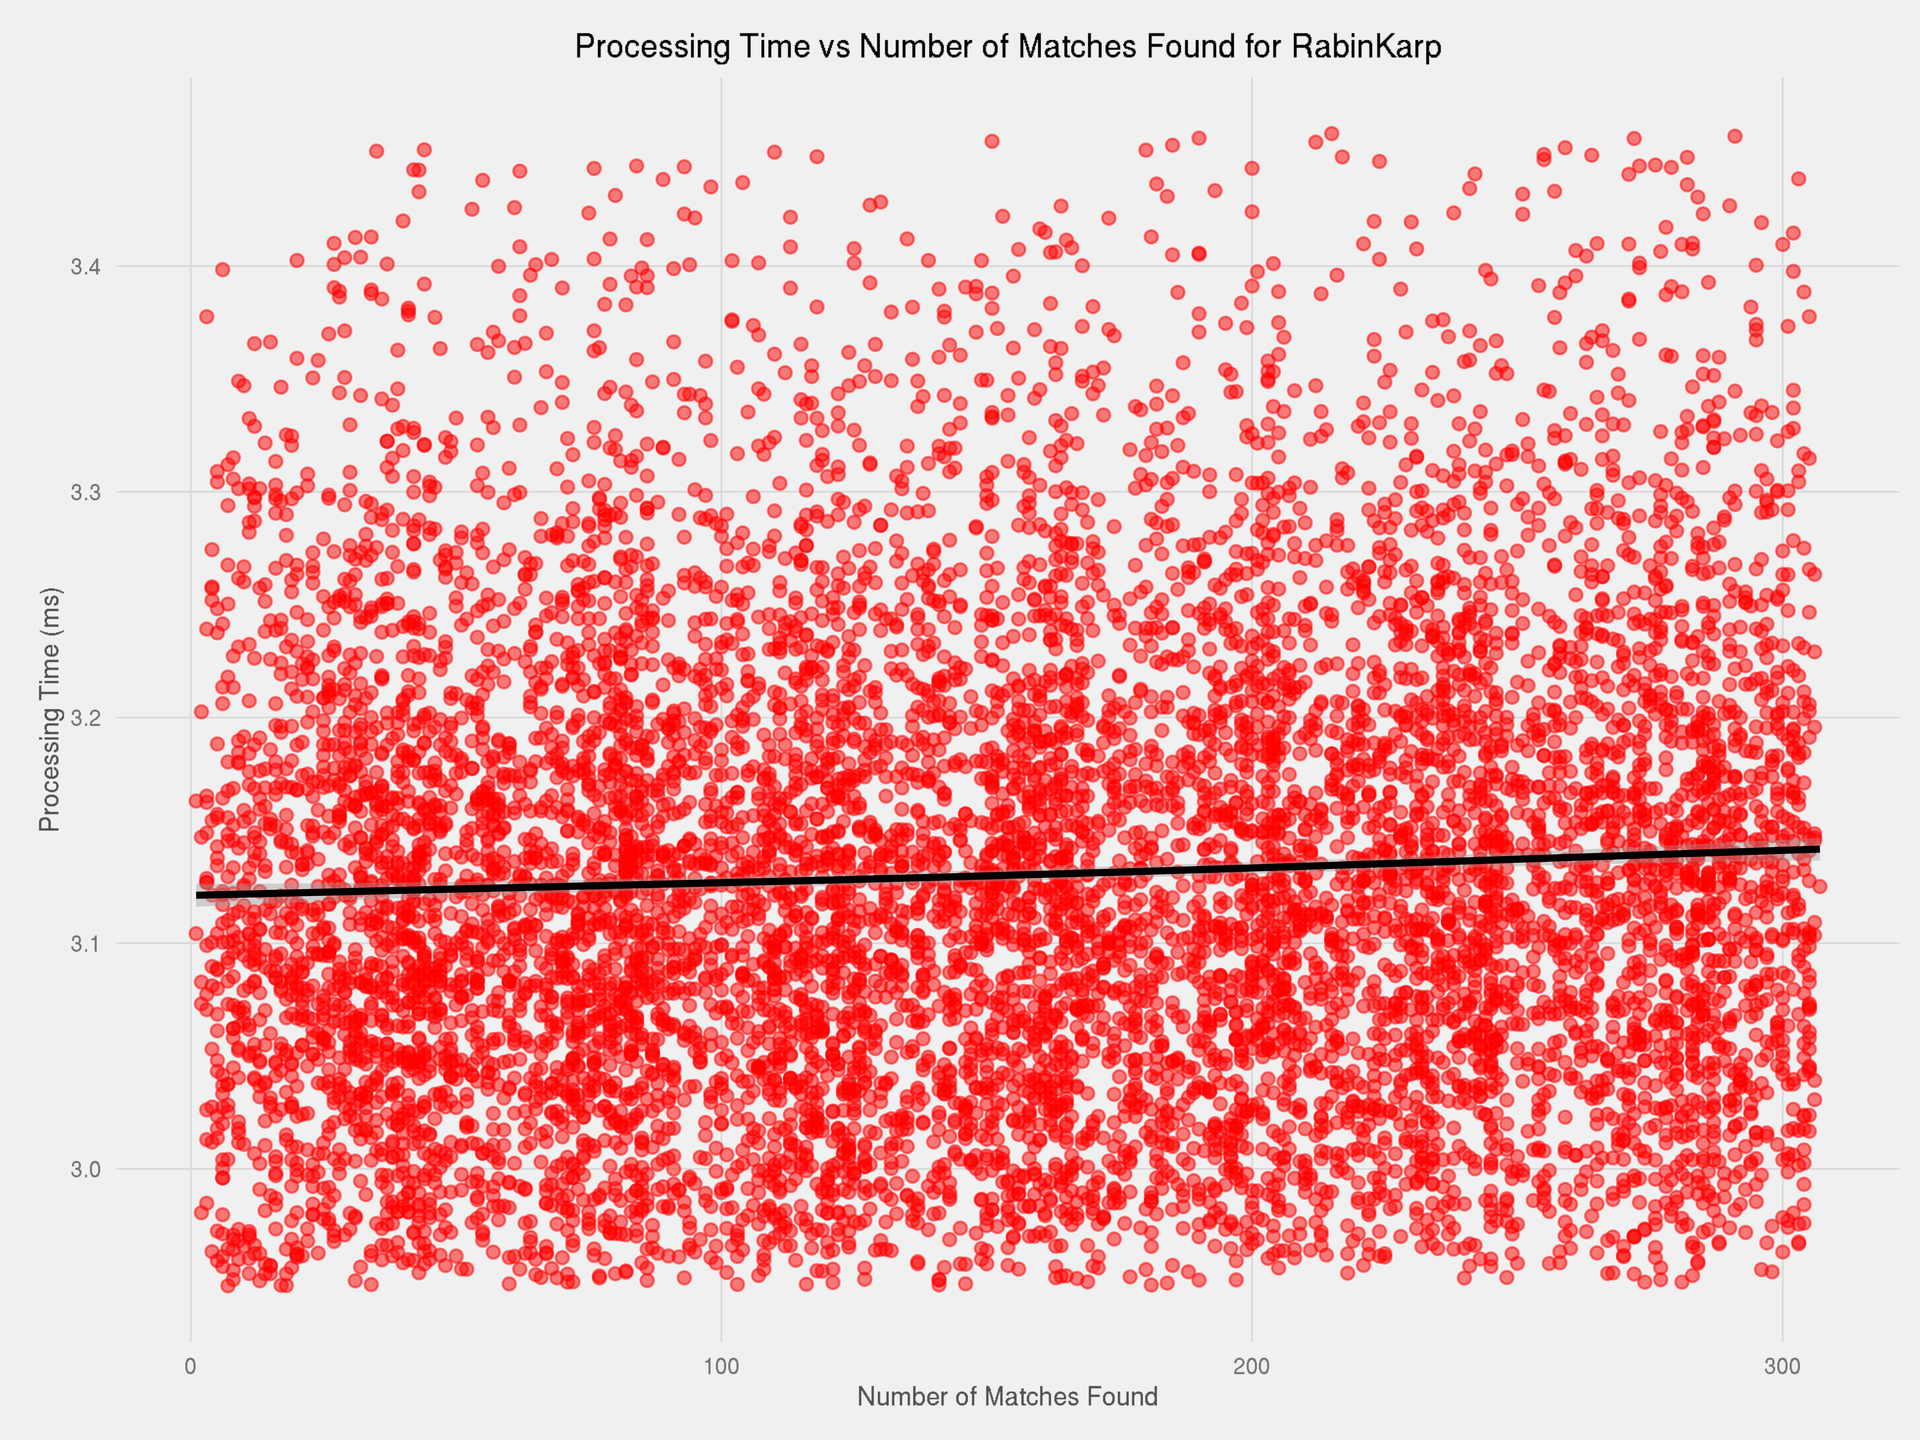
\includegraphics[width=\textwidth]{images/processing_speed_vs_num_matches_RabinKarp}
      \caption{RabinKarp}
  \end{subfigure}
  \caption{Mean processing times for each algorithm vs number of matches. \textit{Dataset F}.}
  \label{figure-individualalgorithmsvsnumberofmatches}
\end{figure}

As can be seen in Figure \ref{figure-individualalgorithmsvsnumberofmatches} the processing speed of both NotSoNaive and RabinKarp seem to not be affected by the number of matches in each packet whereas the number of packets does seem to affect the processing speeds of the Horspool and QuickSearch algorithms. These results make sense. 

The NotSoNaive and RabinKarp algorithms incur little computational penalty when comparing against a substring that matches a rule compared with one that does not. 
Both the Horspool and QuickSearch algorithms make use of BoyerMoore's \citep{boyer1977} bad-character shift table. This table is most effective when few or no matches are present and it allows the algorithms to skip forward over characters which cannot form part of a match. Because \textit{Dataset F} contains so many matches bad-character shift table does not prove to be very useful.


\section{Processing Speed vs Number of Threads}

In order to test how each of the algorithms performs under different levels of parallelism, a simple set of tests was devised. \textit{Dataset C} was selected as the input for the tests as it would not contain any matches to the rules used.  The configuration file mentioned in \citet{hunt2016} allows the number of threads to be specified. The test hardware has a total of 24 cores available and the test searches for each of the rules in parallel. In this test's case there were 40 rules. The following numbers of threads were selected to be tested: 1, 2, 4, 8, 16, 32, 64.

An overall speed increase should take place for thread numbers between one and sixteen. This is still below the twenty four cores available and so each thread can occupy a separate core. At thirty two threads there are now more threads than available cores and so threads have to share processing time on cores. This could lead to further overhead as the processor switches contexts depending on which thread has been scheduled.

\begin{figure}[!htb]
  \centering
  \begin{subfigure}[b]{0.48\textwidth}
      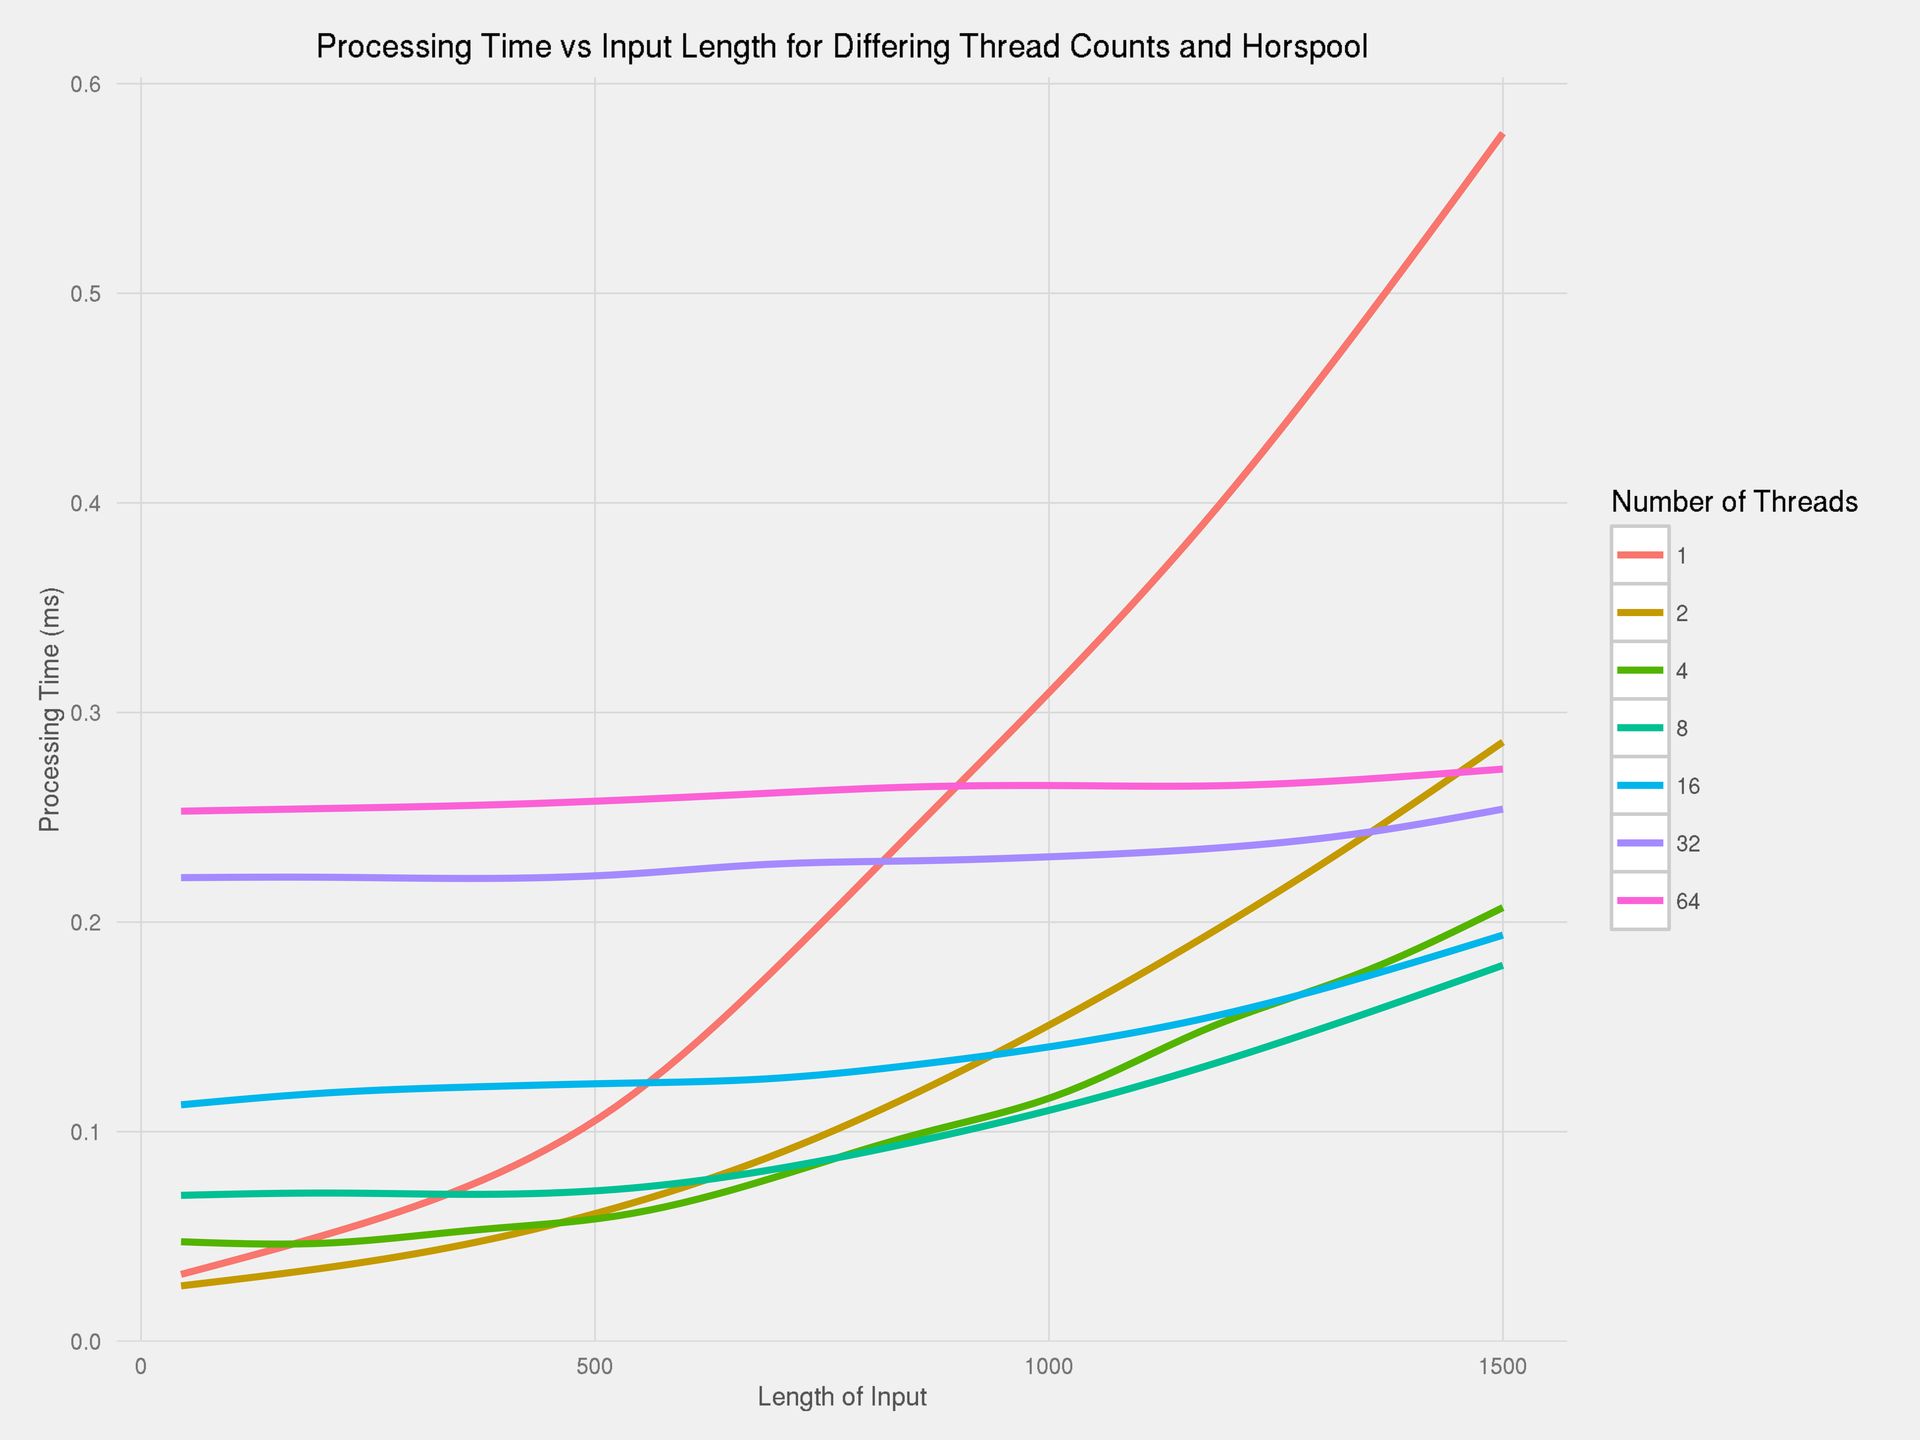
\includegraphics[width=\textwidth]{images/scatter_elapsed_vs_input_length_many_cores_Horspool}
      \caption{Horspool}
  \end{subfigure}
  \begin{subfigure}[b]{0.48\textwidth}
      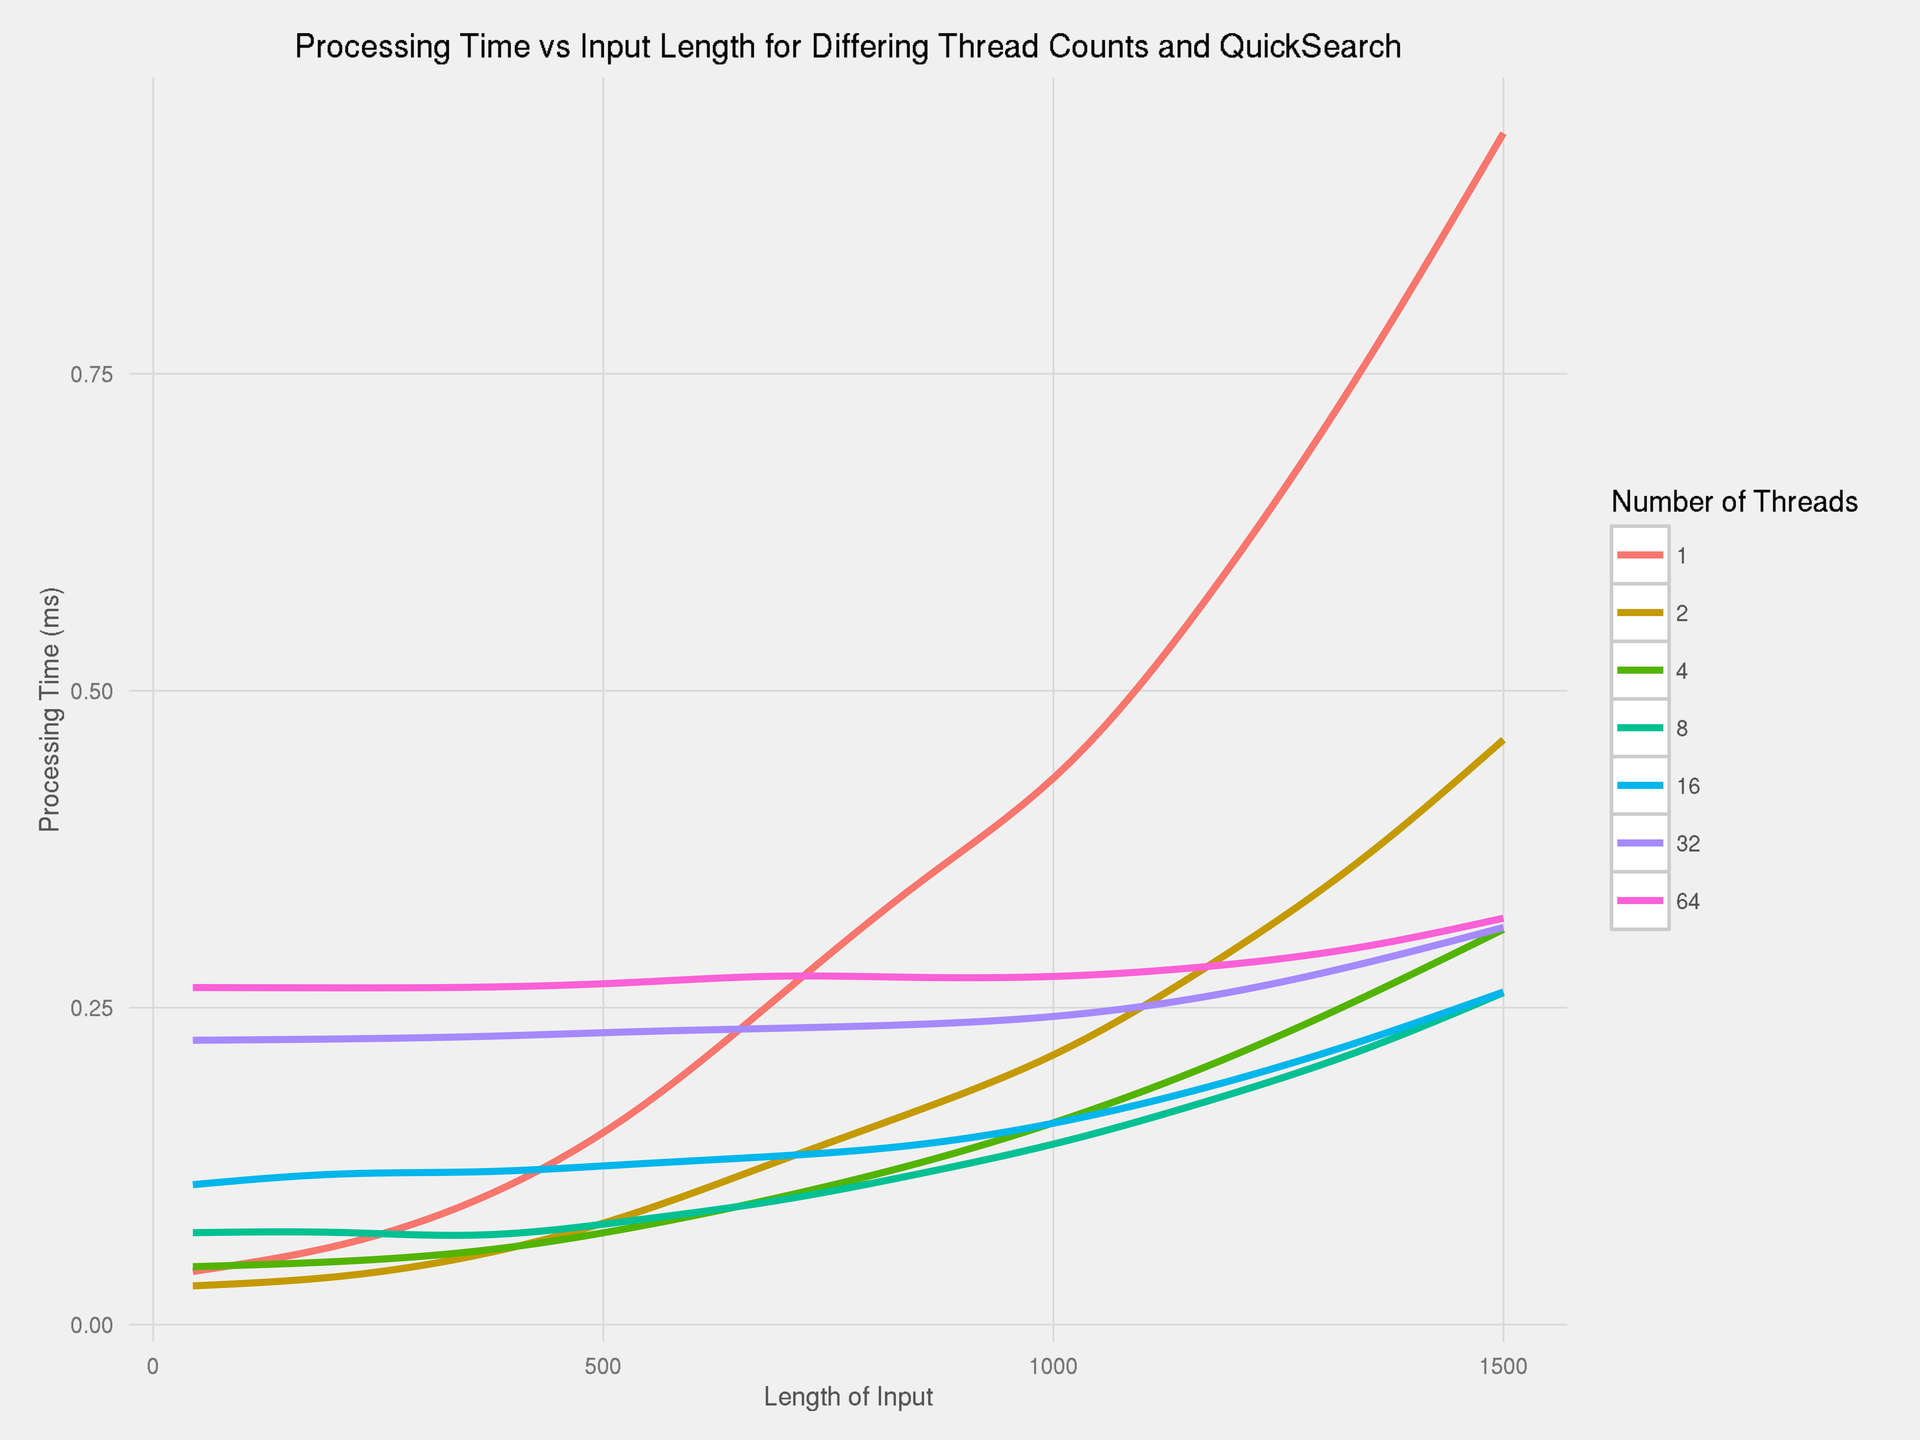
\includegraphics[width=\textwidth]{images/scatter_elapsed_vs_input_length_many_cores_QuickSearch}
      \caption{QuickSearch}
  \end{subfigure}
  ~
  \begin{subfigure}[b]{0.48\textwidth}
      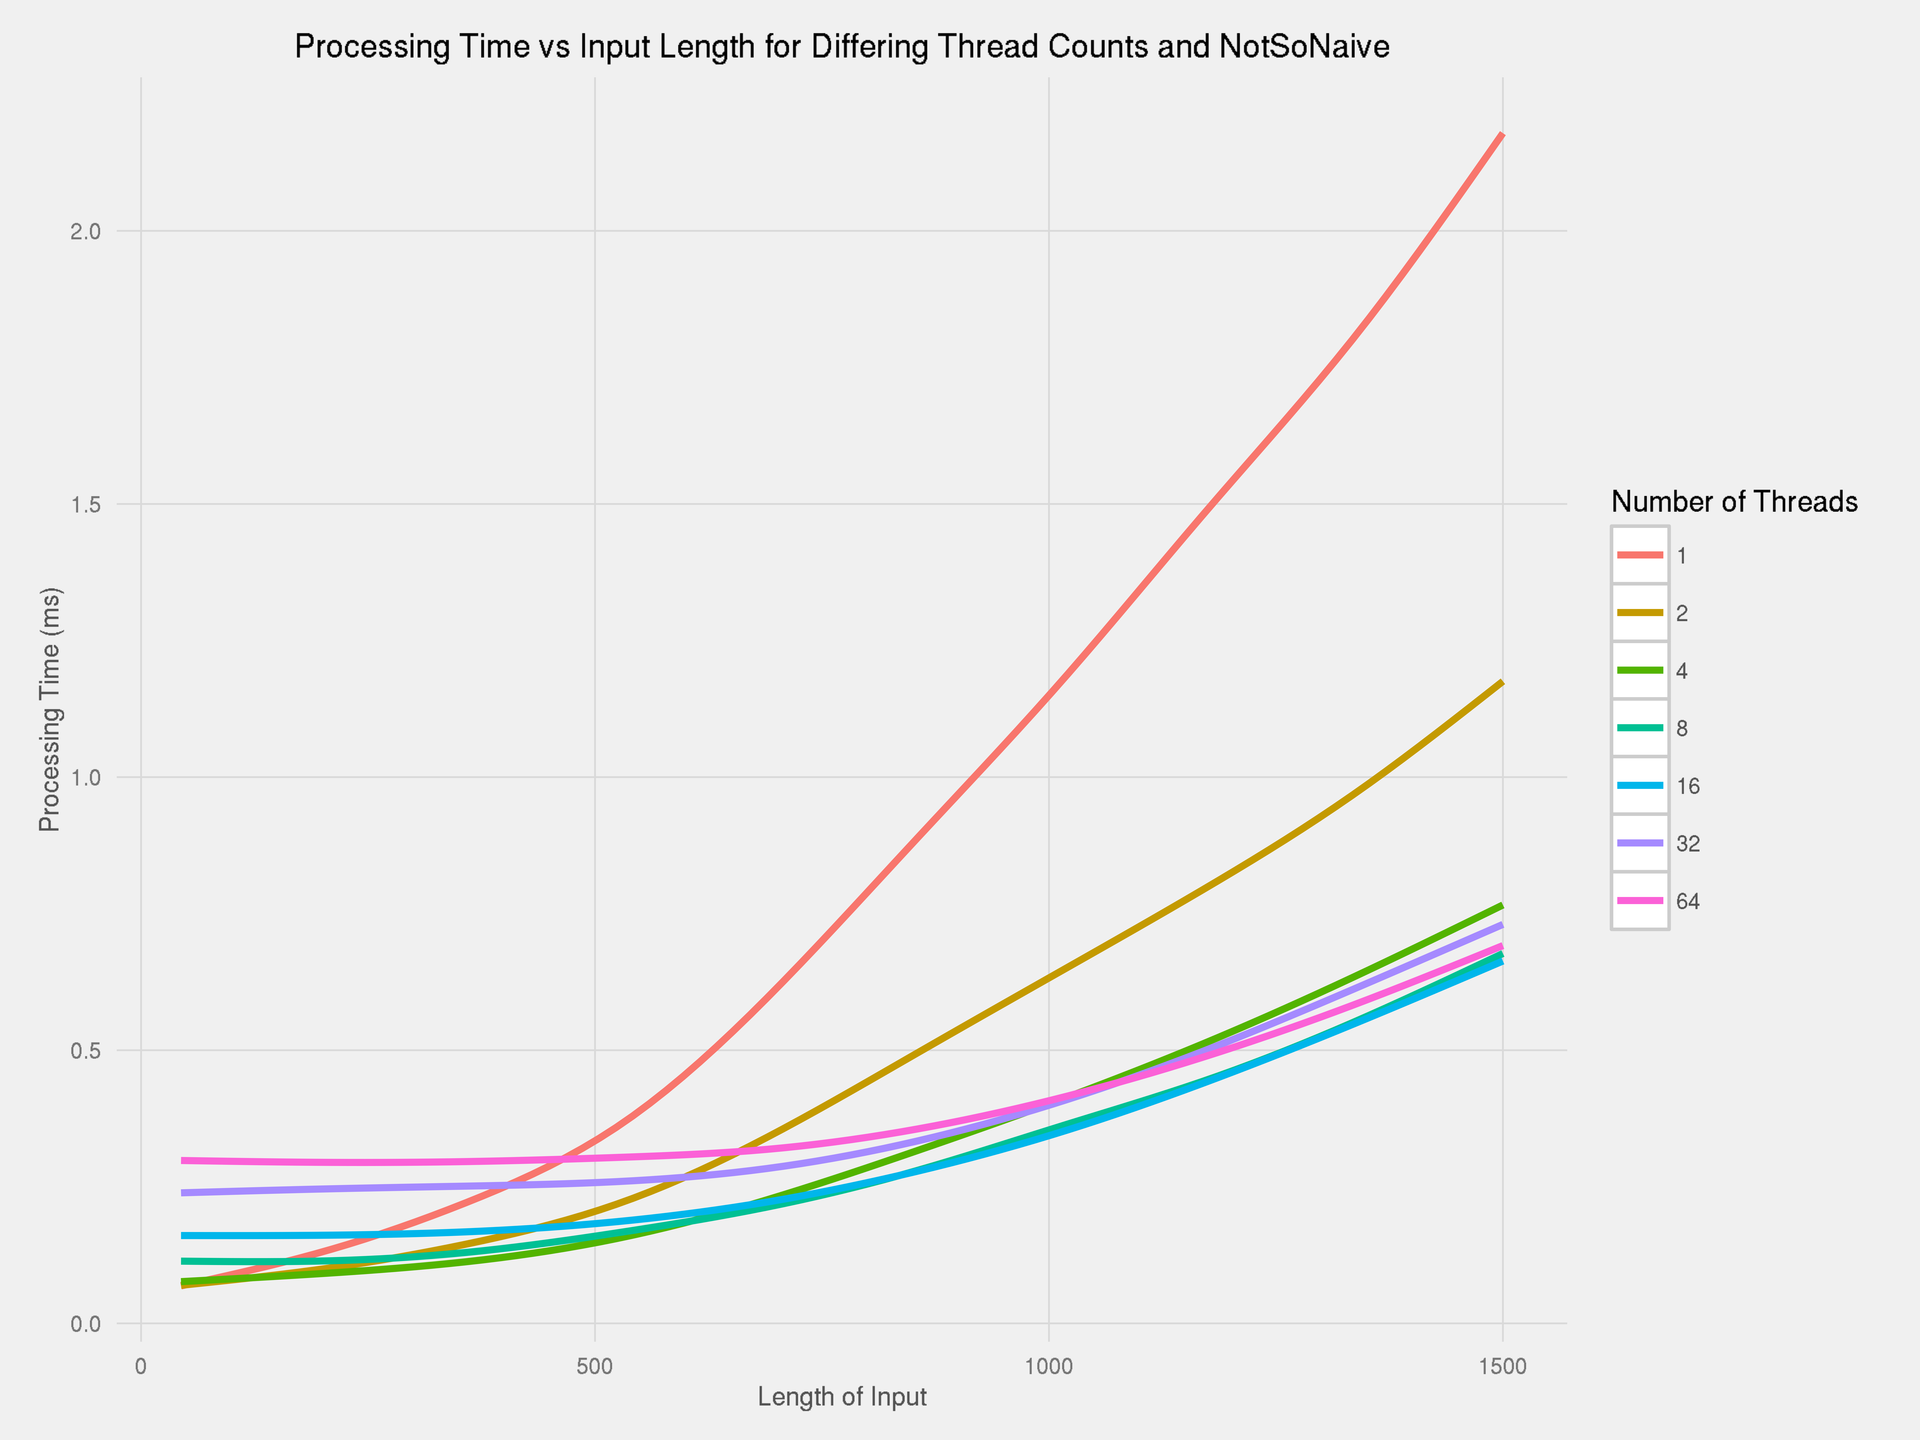
\includegraphics[width=\textwidth]{images/scatter_elapsed_vs_input_length_many_cores_NotSoNaive}
      \caption{NotSoNaive}
  \end{subfigure}
  \begin{subfigure}[b]{0.48\textwidth}
      \includegraphics[width=\textwidth]{images/scatter_elapsed_vs_input_length_many_cores_Rabinkarp}
      \caption{RabinKarp}
  \end{subfigure}
  \caption{Mean processing times for each algorithm vs number of matches. \textit{Dataset D}.}
  \label{figure-processingtimevsinputlengthdifferentcores}
\end{figure}

Figure \ref{figure-processingtimevsinputlengthdifferentcores} provides some very interesting results. As expected, single core implementations are the slowest at longer input lengths and speed increases for more cores are realised as the length of the packets grow. This result is unsurprising as longer packets mean that the overhead of switching threads is diminished as more of the processing time is spent on the searching and less on switching between threads. Also as expected, the lower thread counts are more efficient for smaller packets but they lose efficiency as the length increases. 

On our particular test hardware, between eight and sixteen threads proves to be the most efficient for longer packet lengths. Table \ref{table-threadcompare} shows the outcome of the comparison at various input lengths.


\begin{table}[!htb]
\centering
\begin{tabular}{@{}llll@{}}
\toprule
 & 25\% & 50\% & 75\% \\ \midrule
Horspool & 2 & 4-8 & 8 \\
QuickSearch & 2 & 8 & 8 \\
NotSoNaive & 4 & 8 & 16 \\
RabinKarp & 16 & 16 & 16 \\ \bottomrule
\end{tabular}
\caption{Most efficient number of threads at various percentages of 1500 bytes for each algorithm}
\label{table-threadcompare}
\end{table}

Table \ref{table-threadcompare} shows that for shorter inputs, fewer threads are more efficient. Furthermore, as is apparent in both Figure \ref{figure-processingtimevsinputlengthdifferentcores} and Table \ref{table-threadcompare}, the faster algorithms tend to be more efficient at lessor numbers of threads for the same input lengths as the slower algorithms.

\bibliographystyle{plainnat}
\bibliography{references}

\end{document}